\documentclass[../../../include/open-logic-section]{subfiles}

\begin{document}

\olfileid[hi]{sth}{ordinals}{idea}	
\olsection{क्रमसूचक का सामान्य विचार}

प्राकृतिक संख्याओं पर उनके सामान्य क्रम में विचार करें:
\begin{center}
	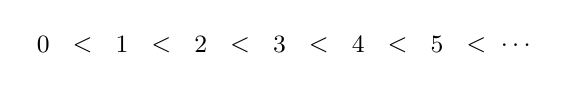
\begin{tikzpicture}
	\foreach \x/\xtext in {0, 1, 2, 3, 4, 5}
	{
		\node (\x a) at (\x, 1) {\small{$\x$}};
		\node (\x a) at (\x.5, 1) {\small{$<$}};
	}
	\node (ldots) at (6, 1) {\small{$\ldots$}};
	\end{tikzpicture}
\end{center}
तकनीकी भाषा में इसे $\omega$-अनुक्रम कहते हैं। वास्तव में यही सामान्य क्रम
समुच्चय पदानुक्रम के चरणों की हमारी आरंभिक रचना में प्रतिबिंबित होता है। अब
मान लें कि हम $0$ को इस अनुक्रम के अंत में ले जाते हैं, ताकि वह अन्य सभी
संख्याओं के बाद आए:
\begin{center}
	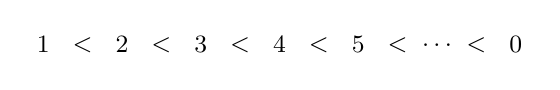
\begin{tikzpicture}
	\foreach \x/\xtext in {1, 2, 3, 4, 5}
	{
		\node (\x a) at (\x, 1) {\small{$\x$}};
		\node (\x a) at (\x.5, 1) {\small{$<$}};
	}
	\node (ldots) at (6, 1) {\small{$\ldots$}};
	\node (bea) at (6.5, 1) {\small{$<$}};
	\node (noa) at (7, 1) {\small{$0$}};
	\end{tikzpicture}
\end{center}
यहाँ वही सत्ताएँ हैं, किंतु मूलतः भिन्न ढंग से क्रमित: हमारे पहले क्रम का
कोई अंतिम अवयव नहीं था; नए क्रम का है। वास्तव में हमारा नया क्रम सत्ताओं के
एक $\omega$-अनुक्रम ($1, 2, 3, 4, 5, \ldots$) और उसके बाद एक अन्य सत्ता
से बना है। यह $\omega+1$-अनुक्रम होगा।

केवल इन्हीं सत्ताओं से हम और भी प्रकार के क्रम बना सकते हैं। उदाहरणतः सभी
सम संख्याओं (उनके स्वाभाविक क्रम में) के बाद सभी विषम संख्याओं (उनके
स्वाभाविक क्रम में) पर विचार करें:
\begin{center}
	\begin{tikzpicture}
	\node(a1) at (1,1) {\small{$0$}};
	\node(a2) at (1.5,1) {\small{$<$}};
	\node(a3) at (2,1) {\small{$2$}};
	\node(a4) at (2.5,1) {\small{$<$}};
	\node(a5) at (3,1) {\small{$4$}};
	\node(a6) at (3.5,1) {\small{$<$}};
	\node(dots) at (4,1) {\small{$\ldots$}};
	\node(aaoe) at (4.5,1) {\small{$<$}};
	\node(b1) at (5,1) {\small{$1$}};
	\node(b2) at (5.5,1) {\small{$<$}};
	\node(b3) at (6,1) {\small{$3$}};
	\node(b4) at (6.5,1) {\small{$<$}};
	\node(b5) at (7,1) {\small{$\ldots$}};
	\end{tikzpicture}
\end{center}
यह एक $\omega$-अनुक्रम के बाद दूसरा $\omega$-अनुक्रम है; एक
$\omega+\omega$-अनुक्रम।

हम इसी तरह आगे बढ़ सकते हैं। किंतु हमें \emph{क्रमों} की इस चर्चा को समझने
का कोई सामान्य ढंग चाहिए।

\end{document}
